\section{Additional Discussion}
\subsection{Testing Sinusoidality of a sample}
Perhps before even going into the task of fitting a \sindist{} to a statistical object, given a sample we should check its goodness of fit to the \sindist{} family. This is possible by usual nonparametric procedures such as the Kolmogorov-Smirnov or the Anderson-Darling test. Like in the case of testing for normality, the algorithm involves first estimating the parameters of the ``best-fitting'' \sindist{} by optimizing an appropriate criterion, such as the joint likelihood. Next, an appropriate non-parametric test is carried out between the fitted density and the observed sample.

In this regard, it is to be noted that the Chi-squared test, which involves binning the observations, before comparing observed and expected frequencies, adds an additional layer of opacity between the sample and the distribution function, by dint of an arbitrary choice of binning. On the other hand, a test like the Shapiro-Wilk test, which depends on specific esoteric properties of the Normal distribution, could not be devised for the \sindist{} as of yet, because no particular identifying property of that sort that can be leveraged similarly has been found yet.

\subsection{Density-quantile domain divergences}
Following \cite{staudte2017dqf}, we may construct the notion of divergences based on the density-quantile function $dq(p) = f(F^{-1}(p)) \quad \forall p \in [0,1]$. A benefit of calculating divergence metrics on the density-quantile domain is that densities (and thereby divergences) are location-scale invariant and invariant to ``flat'' regions in the CDF. However, the computational complexity of evaluating the quantile function of a \sindist{}, and consequent to the same, optimizing with respect to its parameters some functional of the quantile function, is a strong deterrent against this mode of operation.

\begin{comment}
	\subsubsection{DQF on DQF}
\end{comment}


\subsection{Divergence potential map as the determining factor behind fits}
For some target density $g$, if its divergence from any candidate density $f$, $D_g(f) \equiv D(f,g): \mathscr F \times \mathscr G \mapsto \RR$ can often be represented as an integral:
\[\int_{x \in \mathcal X} L(f(x),g(x)) \d x\]
We introduce $V(x,y) = L(y, g(x))$ as the \textbf{divergence density/potential associated with $g$ and induced by $L$}. It gives a glimpse at the topography of penalization of $D(\cdot, \cdot)$ with respect to $g$. Some common divergences with their associated potentials are provided in \autoref{tab:pdfpotlist}. \autoref{fig:dpdpots} gives a visualization of the potential associated with a contaminated density.


\begin{table}[h!]
	\begin{tabular}{c|c|c|c}
		Divergence name  &  Form  &  Potential $L_g(y)$  &  Gradient $\nabla_y L_g(y)$\\
		\hline \vspace{0.1cm}
		
		Hellinger
		&
		$\int \frac{1}{2} (\sqrt{y(x)} - \sqrt{g(x)})^2 \d x$
		&
		$\frac{1}{2} (\sqrt y - \sqrt g)^2$
		&
		$\frac{1}{2 \sqrt y} (\sqrt y - \sqrt g)$
		\\
		
		DPD-\texorpdfstring{$\alpha$}{alpha}
		&
		$\int y^\alpha(y-g) - \frac{1}{\alpha}g(y^\alpha - g^\alpha) \d x$
		&
		$y^\alpha(y-g) - \frac{1}{\alpha}g(y^\alpha - g^\alpha)$
		&
		$(1+\alpha) y^{\alpha-1} (y-g)$
		\\
		
		Kullback--Leibler
		&
		$\int y \log \left(\frac{y}{g}\right) \d x$
		&
		$y \log \left(\frac{y}{g}\right)$
		&
		$\log \left(\frac{y}{g}\right) + 1$
		\\
		
		Reverse KL
		&
		$\int g \log \left(\frac{g}{y}\right) \d x$
		&
		$g \log \left(\frac{g}{y}\right)$
		&
		$-\frac{g}{y}$
		\\
		
		Pearson $\chi^2$
		&
		$\int \frac{(y-g)^2}{g} \d x$
		&
		$\frac{(y-g)^2}{g}$
		&
		$\frac{2(y-g)}{g}$
		\\
		
		Neyman $\chi^2$
		&
		$\int \frac{(y-g)^2}{y} \d x$
		&
		$\frac{(y-g)^2}{y}$
		&
		$1-\frac{g^2}{y^2}$
		\\
		
		Total variation
		&
		$\int |y-g| \d x$
		&
		$|y-g|$
		&
		$\mathrm{sign}(y-g)$
		\\
		
		Jensen--Shannon
		&
		$\frac12 \int \left[ y \log \left(\frac{2y}{y+g}\right)
		+ g \log \left(\frac{2g}{y+g}\right) \right]\d x$
		&
		$\frac12 y \log \left(\frac{2y}{y+g}\right)
		+\frac12 g \log \left(\frac{2g}{y+g}\right)$
		&
		$\frac12 \log \left(\frac{2y}{y+g}\right)$
		\\
		
	\end{tabular}
	\caption{Some common PDF-PDF divergences and their potential functions}
	\label{tab:pdfpotlist}
\end{table}

Note how almost all divergences are functions of $f-g$, i.e. dependent on the abscissa-wise deviation of the candidate density from the target. However the rate of increment of penalization wrt. the deviation changes with the divergences.

The process of fitting a candidate distribution over a given target then becomes merely an act of minimizing the integral of potential along the density-line, with the constraint of area under the density line as 1.

\subsubsection{DPD and contamination}
To understand the influence of the tuning parameter $\alpha$ on the DPD metric, with the ambition of suggesting novel ways of estimating the same, a long-standing research question (\cite{basak2021dpd}), we observe heuristically that a higher $\alpha$ causes a lower rate of increase of penalization for deviating from true curve, thereby providing more feasibility of a fit that covers both density portions. Whereas a lower $\alpha$ allows rigid maximization over one of the 2 curves only, since passing through the middle high-penalization region in between incurs a lot of cost. See \autoref{fig:dpdpots}.

   \begin{figure}[h]
   	\centering
	\begin{subfigure}{0.49\linewidth}
		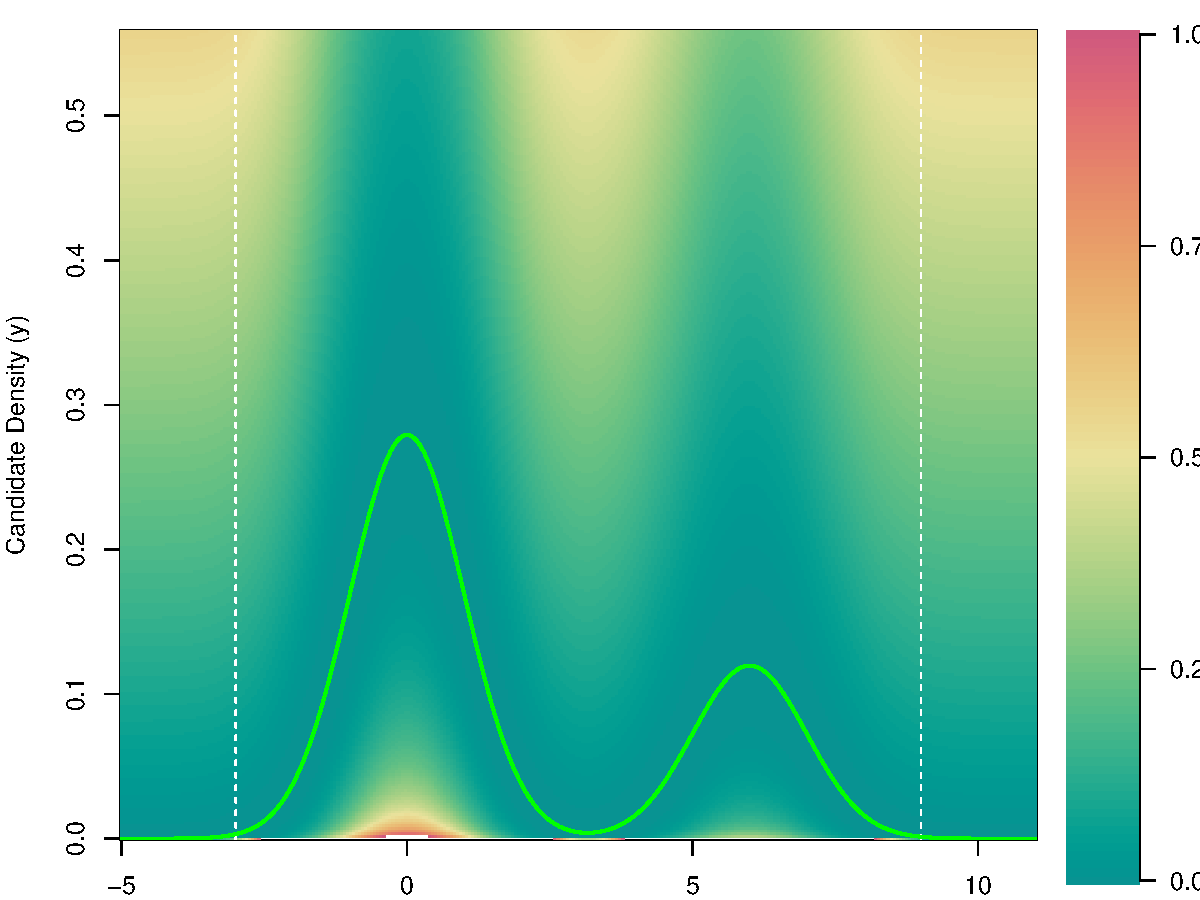
\includegraphics[width=\linewidth]{fig/divpot contamin 0.01}
		\caption{$\alpha=0.01$}
	\end{subfigure}
	\begin{subfigure}{0.49\linewidth}
		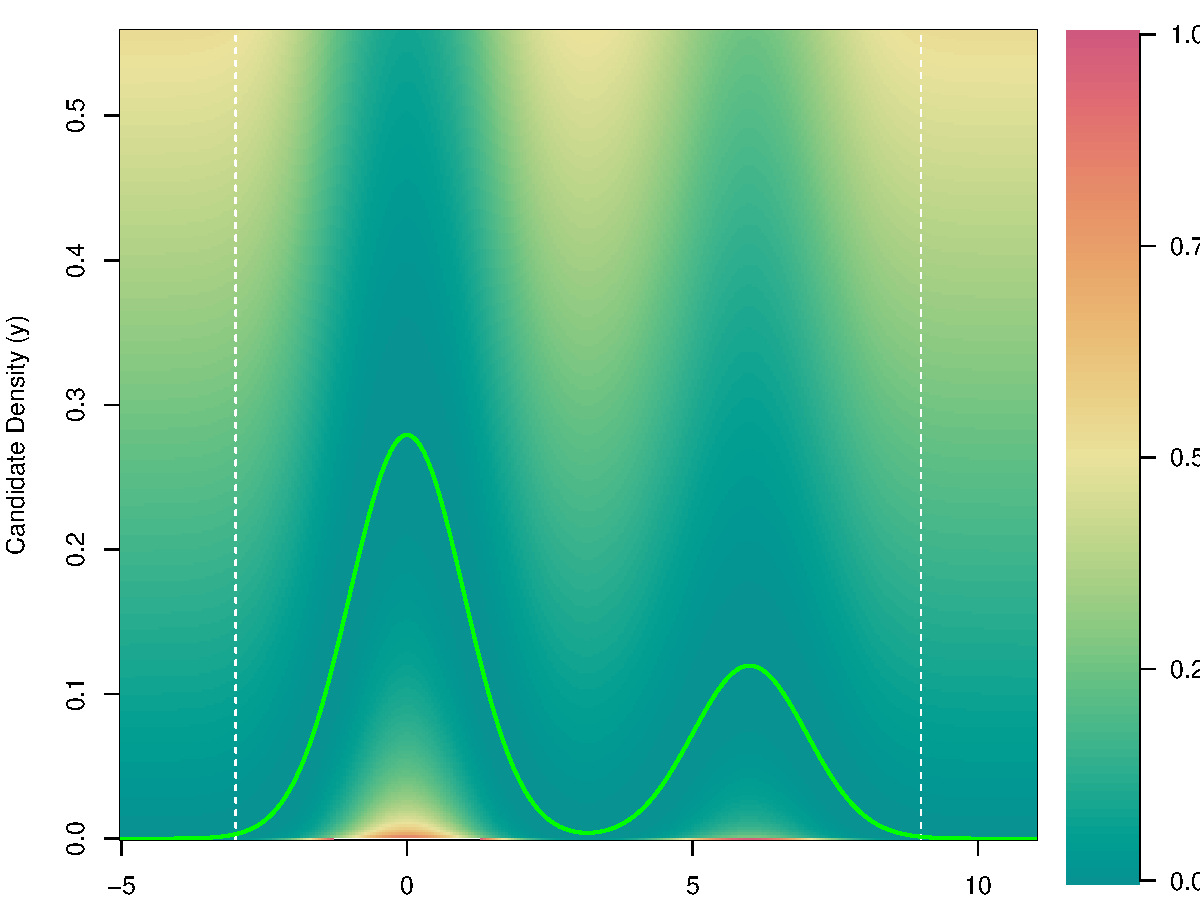
\includegraphics[width=\linewidth]{fig/divpot contamin 0.1}
		\caption{$\alpha=0.1$}
	\end{subfigure}
	\begin{subfigure}{0.49\linewidth}
		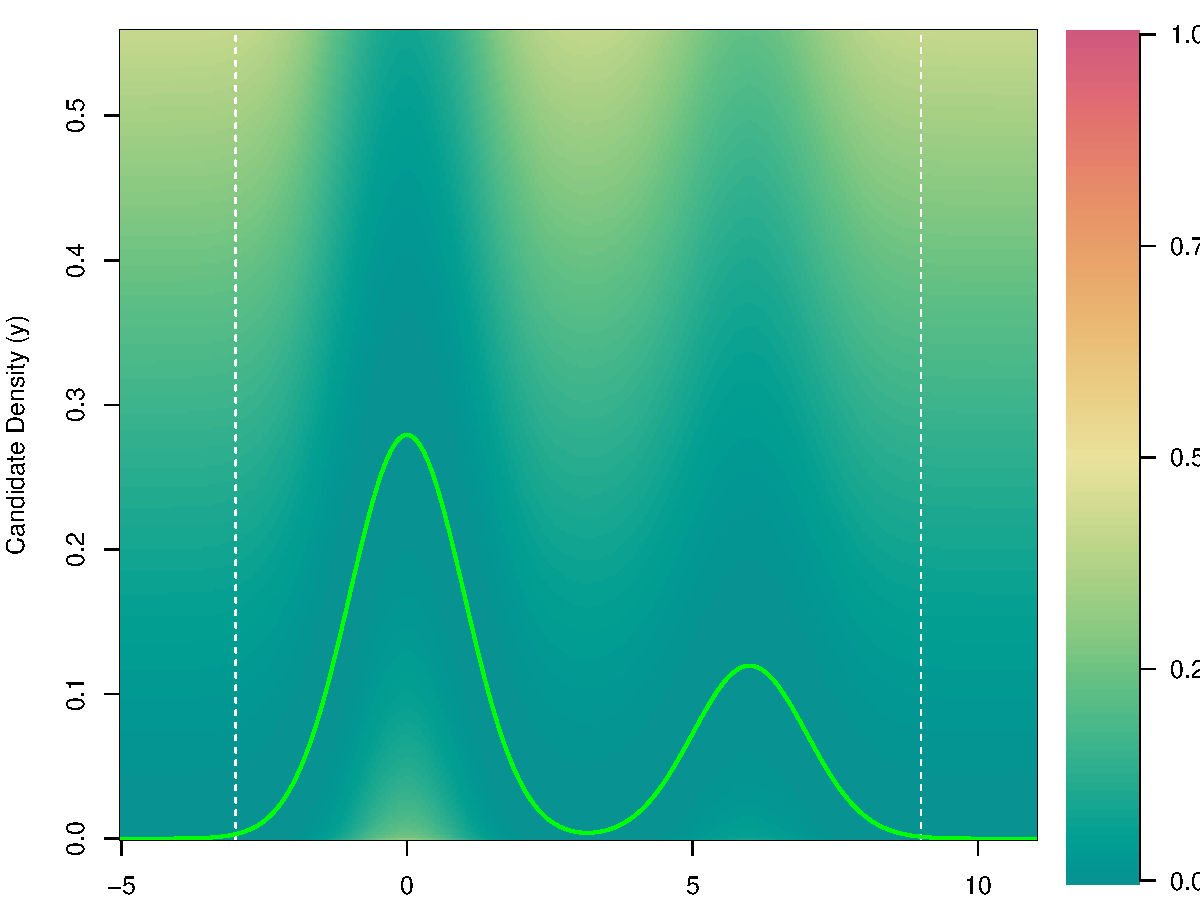
\includegraphics[width=\linewidth]{fig/divpot contamin 0.5}
		\caption{$\alpha = 0.5$}
	\end{subfigure}
	\begin{subfigure}{0.49\linewidth}
		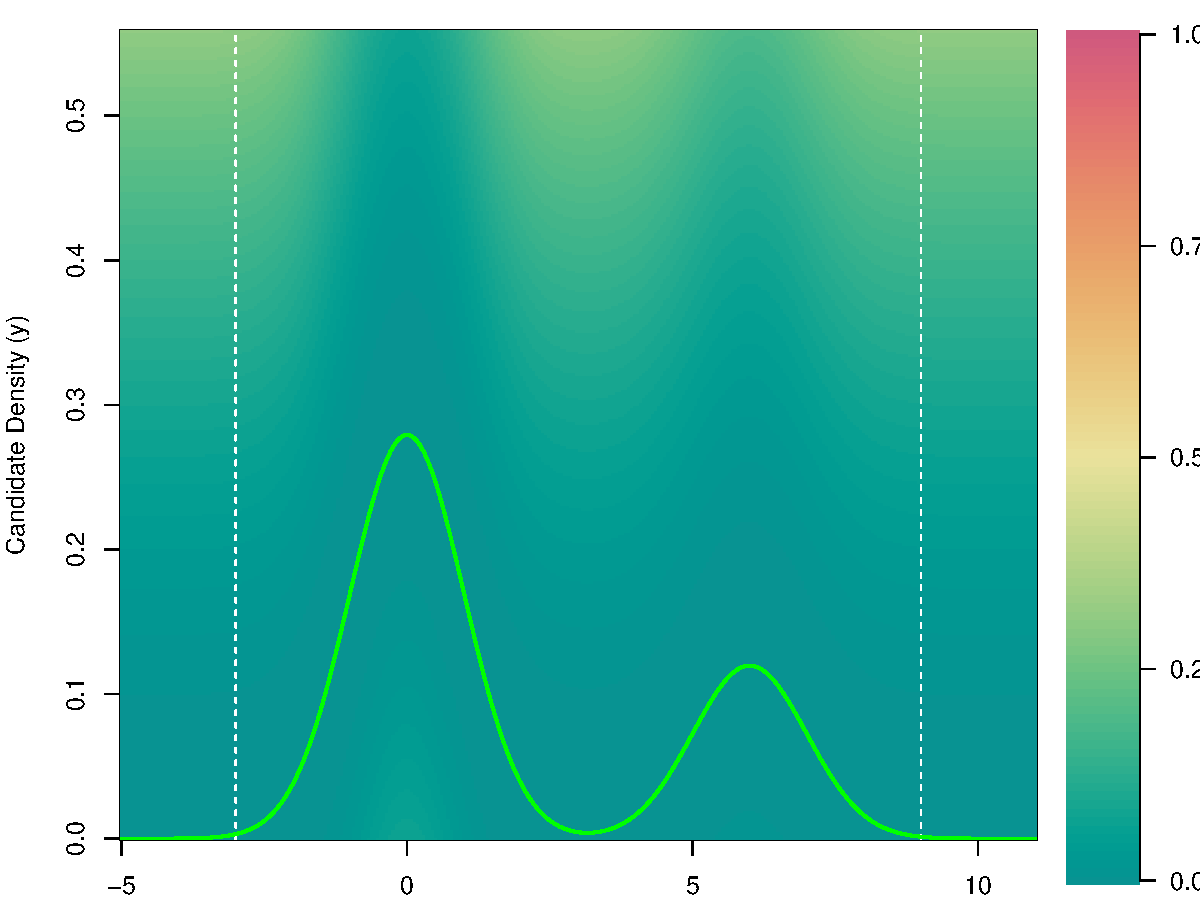
\includegraphics[width=\linewidth]{fig/divpot contamin 1}
		\caption{$\alpha = 1$}
	\end{subfigure}
	\caption{Divergence potentials induced by different $\alpha$'s of the contaminated density $0.7 \N(0,1) + 0.3 \N(0, 1)$}\label{fig:dpdpots}
\end{figure}

We find that for contaminated densities, it is not the ``attraction'' of the second peak that deviates the candidate to fit contaminatedly, but it is the infeasibility in between that makes unimodal densities suboptimal fits, thereby seeking that the candidate choose either the principal or the contaminant density component.

\begin{comment}
	In the presence of contamination, there is the additional complexity of the principal density being scaled down. So even if the distribution were to fit to the principal density portion, it would it to a dwarved version of it, thereby adjusting a best fit over its ``cloud" of minimality. Thereby the candidate distribution is now betrayed to fit over a ``non-density" principal component.
	
	We can conclude that the \sindist{} is indeed more flexible if for different target densities, which may even come from data, it can minimize the divergence better than conventional distributions. At the same time, excess efficiency implies lack of robustness in the presence of contamination. In such cases, we justify the utility of the \sindist{} by saying that it fits to data more flexibly than other distributions, and transparently displays the nature of the underlying divergence metric without interference from the rigidity of its shape.
\end{comment}
